\documentclass[tikz,border=10pt]{standalone}
\usepackage{amsmath}
\usepackage{amssymb}
\usetikzlibrary{arrows.meta, positioning, calc}

\begin{document}
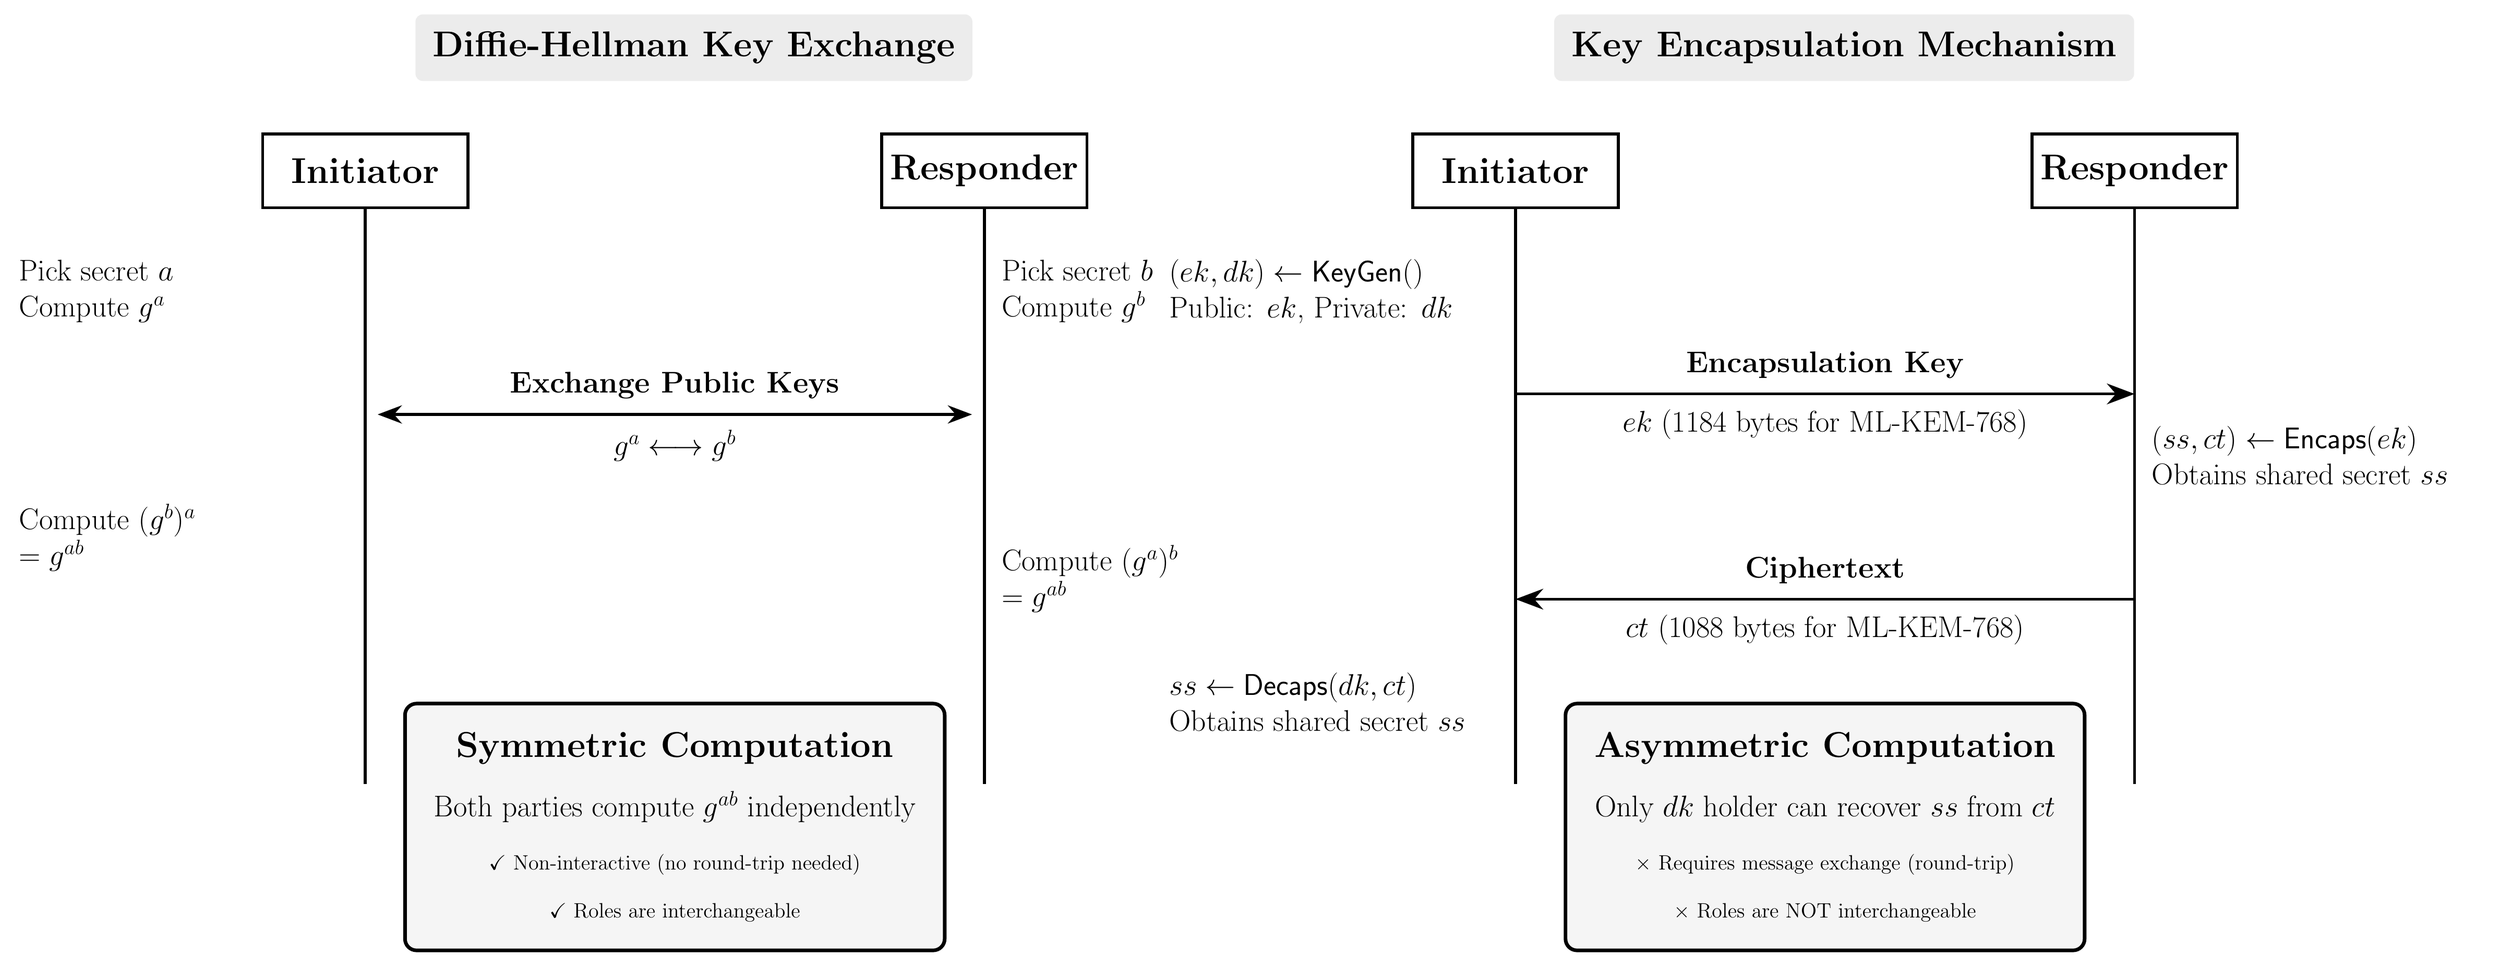
\begin{tikzpicture}[
    box/.style={rectangle, draw=black, line width=2pt, minimum width=5cm, minimum height=1.8cm, align=center, font=\bfseries\Huge},
    arrow/.style={-{Stealth[scale=1.6]}, line width=2pt},
    doublearrow/.style={{Stealth[scale=1.4]}-{Stealth[scale=1.4]}, line width=2pt},
    msg_label/.style={font=\huge\bfseries, fill=white, inner sep=5pt},
    msg_detail/.style={font=\huge, fill=white, inner sep=5pt},
    action/.style={font=\huge, text width=8cm, align=left},
    timeline/.style={line width=2pt},
    section_title/.style={font=\Huge\bfseries, fill=gray!15, rounded corners=5pt, inner sep=12pt},
    result_box/.style={draw, line width=2.5pt, fill=gray!8, rounded corners=8pt, align=center, inner sep=20pt, font=\huge}
]
    % ========== LEFT SIDE: Diffie-Hellman ==========
    \def\colsep{10cm}
    \def\sidesep{28cm}
    
    % DH Title
    \node[section_title] (dh_title) at (8cm, 3cm) {Diffie-Hellman Key Exchange};
    
    % DH Parties
    \node[box] (dh_init) at (0, 0) {Initiator};
    \node[box, right=\colsep of dh_init] (dh_resp) {Responder};
    
    % DH Timelines
    \draw[timeline] (dh_init.south) -- +(0,-14cm);
    \draw[timeline] (dh_resp.south) -- +(0,-14cm);
    
    % DH Row 1: Both generate keypairs (symmetric action)
    \coordinate (dh_r1a) at ($(dh_init.south)-(0,2cm)$);
    \coordinate (dh_r1b) at ($(dh_resp.south)-(0,2cm)$);
    \node[action, anchor=east] at ($(dh_r1a)+(-0.3cm,0)$) {Pick secret $a$\\Compute $g^a$};
    \node[action, anchor=west] at ($(dh_r1b)+(0.3cm,0)$) {Pick secret $b$\\Compute $g^b$};
    
    % DH Row 2: Exchange public keys (bidirectional)
    \coordinate (dh_m1_start) at ($(dh_init.south)-(0,5cm)$);
    \coordinate (dh_m1_end) at ($(dh_resp.south)-(0,5cm)$);
    \draw[doublearrow] ($(dh_m1_start)+(0.3cm,0)$) -- ($(dh_m1_end)-(0.3cm,0)$);
    \node[msg_label, above=0.2cm] at ($(dh_m1_start)!0.5!(dh_m1_end)$) {Exchange Public Keys};
    \node[msg_detail, below=0.2cm] at ($(dh_m1_start)!0.5!(dh_m1_end)$) {$g^a \longleftrightarrow g^b$};
    
    % DH Row 3: Both compute shared secret (symmetric)
    \coordinate (dh_r3a) at ($(dh_init.south)-(0,8cm)$);
    \coordinate (dh_r3b) at ($(dh_resp.south)-(0,9cm)$);
    \node[action, anchor=east] at ($(dh_r3a)+(-0.3cm,0)$) {Compute $(g^b)^a$\\$= g^{ab}$};
    \node[action, anchor=west] at ($(dh_r3b)+(0.3cm,0)$) {Compute $(g^a)^b$\\$= g^{ab}$};
    
    % DH Result box
    \node[result_box, below=12cm of $(dh_init.south)!0.5!(dh_resp.south)$] (dh_result) {
        \textbf{\Huge Symmetric Computation}\\[16pt]
        Both parties compute $g^{ab}$ independently\\[12pt]
        {\Large $\checkmark$ Non-interactive (no round-trip needed)}\\[8pt]
        {\Large $\checkmark$ Roles are interchangeable}
    };
    
    % ========== RIGHT SIDE: KEM ==========
    
    % KEM Title
    \node[section_title] (kem_title) at ($(dh_title)+(\sidesep,0)$) {Key Encapsulation Mechanism};
    
    % KEM Parties
    \node[box] (kem_init) at (\sidesep, 0) {Initiator};
    \node[box, right=\colsep of kem_init] (kem_resp) {Responder};
    
    % KEM Timelines
    \draw[timeline] (kem_init.south) -- +(0,-14cm);
    \draw[timeline] (kem_resp.south) -- +(0,-14cm);
    
    % KEM Row 1: Initiator generates keypair (asymmetric!)
    \coordinate (kem_r1a) at ($(kem_init.south)-(0,2cm)$);
    \node[action, anchor=east] at ($(kem_r1a)+(-0.3cm,0)$) {$(ek, dk) \gets \textsf{KeyGen}()$\\Public: $ek$, Private: $dk$};

    % KEM Row 2: Initiator sends encapsulation key
    \coordinate (kem_m1_start) at ($(kem_init.south)-(0,4.5cm)$);
    \coordinate (kem_m1_end) at ($(kem_resp.south)-(0,4.5cm)$);
    \draw[arrow] (kem_m1_start) -- (kem_m1_end);
    \node[msg_label, above=0.2cm] at ($(kem_m1_start)!0.5!(kem_m1_end)$) {Encapsulation Key};
    \node[msg_detail, below=0.2cm] at ($(kem_m1_start)!0.5!(kem_m1_end)$) {$ek$ (1184 bytes for ML-KEM-768)};

    % KEM Row 3: Responder encapsulates
    \coordinate (kem_r3b) at ($(kem_resp.south)-(0,6cm)$);
    \node[action, anchor=west] at ($(kem_r3b)+(0.3cm,0)$) {$(ss, ct) \gets \textsf{Encaps}(ek)$\\Obtains shared secret $ss$};

    % KEM Row 4: Responder sends ciphertext
    \coordinate (kem_m2_start) at ($(kem_resp.south)-(0,9.5cm)$);
    \coordinate (kem_m2_end) at ($(kem_init.south)-(0,9.5cm)$);
    \draw[arrow] (kem_m2_start) -- (kem_m2_end);
    \node[msg_label, above=0.2cm] at ($(kem_m2_start)!0.5!(kem_m2_end)$) {Ciphertext};
    \node[msg_detail, below=0.2cm] at ($(kem_m2_start)!0.5!(kem_m2_end)$) {$ct$ (1088 bytes for ML-KEM-768)};

    % KEM Row 5: Initiator decapsulates
    \coordinate (kem_r5a) at ($(kem_init.south)-(0,12cm)$);
    \node[action, anchor=east] at ($(kem_r5a)+(-0.3cm,0)$) {$ss \gets \textsf{Decaps}(dk, ct)$\\Obtains shared secret $ss$};
    
    % KEM Result box
    \node[result_box, below=12cm of $(kem_init.south)!0.5!(kem_resp.south)$] (kem_result) {
        \textbf{\Huge Asymmetric Computation}\\[16pt]
        Only $dk$ holder can recover $ss$ from $ct$\\[12pt]
        {\Large $\times$ Requires message exchange (round-trip)}\\[8pt]
        {\Large $\times$ Roles are NOT interchangeable}
    };

\end{tikzpicture}
\end{document}
